% !TEX TS-program = xelatex
% !TEX encoding = UTF-8 Unicode

% This is a simple template for a LaTeX document using the "article" class.
% See "book", "report", "letter" for other types of document.

\documentclass[11pt]{article}

\usepackage[margin=1in]{geometry}
\usepackage{fancyhdr}

\usepackage{parskip}
\usepackage{framed}
\usepackage{amsmath,amsthm,amssymb}

\newtheorem*{conjecture}{Conjecture}

\usepackage{titlesec}

\usepackage[svgnames]{xcolor}

%\usepackage{enumerate}
\usepackage{enumitem}
\newcounter{descriptcount}


%\usepackage{mathpazo}
\usepackage{mathtools}
\usepackage{unicode-math}
\usepackage{empheq}
\usepackage[most]{tcolorbox}

\usepackage{caption}

\usepackage{xunicode} %handle unicode
\usepackage{xltxtra} %XeTeX extras
\usepackage{fontspec} %use OTF/TTF fonts

%\newcommand{\lmr}{\fontfamily{lmr}\selectfont} % Latin Modern Roman


%\setmainfont{Myriad Pro} %use this font
%\setmathfont{Adobe Garamond Pro} %use this font for math

\titleformat{\section}
  {\large\bf}{\thesection}{0.25em}{}[\titlerule]
\titlespacing{\section}
  {0pt}{*1.5}{0.25em}

\titleformat{\subsection}
  {\normalfont\bf}{\thesubsection}{0.25em}{}
\titlespacing{\subsection}
  {0pt}{*1}{0.125em}

\renewcommand\thesection{\Alph{section}.}
\renewcommand\thesubsection{\thesection\arabic{subsection}}
\renewcommand\thesubsubsection{(\roman{subsubsection}).}

\renewcommand{\labelitemi}{\textemdash}

\DeclareMathOperator{\dif}{d\!}
%\DeclareMathOperator{\Pr}{P}
\DeclareMathOperator{\E}{E}
\DeclareMathOperator{\var}{var}
\DeclareMathOperator{\F}{\mathfrak{F}}
\DeclareMathOperator{\Poisson}{Poisson}
\DeclareMathOperator{\Bernoulli}{Bernoulli}
\DeclareMathOperator{\Binomial}{Binomial}
\DeclareMathOperator{\Order}{O}
\DeclareMathOperator{\Uniform}{Uniform}
\DeclareMathOperator*{\argmax}{argmax}
\DeclareMathOperator{\Tr}{Tr}

\newcommand{\logdet}[1]{\log \left| {#1} \right| }

\newcommand{\xb}{\mathbf{x}}
\newcommand{\ub}{\symbf{\mu}}
\newcommand{\Sb}{\symbf{\Sigma}}

\newcommand*{\tran}{^{\mkern-1.5mu\mathsf{T}}}
\newcommand*{\invtran}{^{\mkern-1.5mu\mathsf{-T}}}


\newenvironment{propertybox}{%
   \def\FrameCommand{\colorbox{LightSteelBlue}}%
   \MakeFramed{\advance\hsize-\width \FrameRestore}}
 {\endMakeFramed}

\lhead{\textbf{ELEC548}}
\chead{Mixture Models and Expectation Maximization}
\cfoot{}
\rhead{}
\rfoot{\thepage}
\pagestyle{fancyplain}

%\setlength\parindent{0pt}

\allowdisplaybreaks


\begin{document}
\setmainfont{Myriad Pro} %use this font
%\setmathfont{Latin Modern Math}
%\setmathfont{TG Pagella Math}

\begin{center}
\large
\textbf{ELEC 548} Mixture Models and Expectation Maximization
\end{center}

\section{Gaussian Mixtures}
In general, a \textit{mixture model} can be defined for arbitrary probability
distributions. However as is almost always the case, the Gaussian distribution makes
everything work nicely. Mixture models are a key foundation for machine learning based
on probabilistic generative models.

We will use a \textit{Mixture of Guassians} as a probabilistic generative model
for clustering. A good reference for this topic is Chapter 9 of Bishop's
\textit{Pattern Recognition and Machine Learning}. The first step to generate
a data point is to start with the cluster identity.

\begin{flalign*}
  \text{Let} \; z \in \lbrace 1, \ldots, K\rbrace \;
  \text{be a discrete random variable.} &
\end{flalign*}

We can define the probability of drawing a point from an individual mixture component
(i.e., cluster) as

\begin{equation}
\Pr(z = k) = \pi_k, \; \text{where} \; k = 1, \ldots, K.
\end{equation}

Note that for $\Pr(z)$ to be a valid probability distribution, $0 \leq \pi_k
\leq 1$ and $\sum_{k = 1}^{K} \pi_k = 1$.

\begin{propertybox}
\textbf{Aside:} We have begun our discussion of mixture models implicitly
assuming that the number of cluters, $K$, is specified. Non-parametric models,
for which $K$ would not be prespefied, have been an area of active development
in the last decade. A good introduction to this topic is Chapter 25 of Murphy
\textit{Machine Learning: A Probabilistic Perspective}.
\end{propertybox}

Once we have our \textit{prior probability}, $\Pr(z)$, we can define the
distribution of the data point from the selected mixture component

\begin{equation}
\Pr(\xb \mid z = k) = \mathcal{N} (\xb \mid \ub_k, \Sb_k)
\end{equation}

Combining the prior probability of the cluster and the distribution of data
points within the cluster we get the marginal probability of an observed data
point:

\begin{equation}
\Pr(\xb) = \sum_{z} \Pr(\xb \mid z) \Pr(z)
         = \sum_{k=1}^K \mathcal{N} (\xb \mid \ub_k, \Sb_k) \pi_k.
\end{equation}

{\bf A peak ahead:} We will use the $\Pr(\xb)$ density with training data to do
\textbf{ maximum likelihood parameter estimation}. Then, with optimized
parameters we can use the \textit{a posteriori} density, $\Pr(z \mid \xb)$, to
assign data points to clusters either with a ``''hard decision'' (choosing the
class which maximizes the density) or with a ``soft decision'' (keeping track of
how likely the datapoint is to have come from each cluster).

\subsection{Maximum likelihood parameter estimation}
\begin{flalign*}
  \text{\bf Goal:} \quad \text{Fit} \; \ub_k, \Sb_k, \pi_k \; \text{to training data} \;
      \xb_1, \ldots, \xb_N. &
\end{flalign*}

We will use the notational shorthand $\lbrace \xb \rbrace$ for the training data
$\xb_1, \ldots \xb_N$, and the shorthand $\theta$ for all the parameters of the
model $\lbrace \ub_k, \Sb_k, \pi_k\rbrace_{k = 1, \ldots, K}$. Then, we can
write down the likelihood of our training data
\begin{align*}
	\Pr (\lbrace \xb \rbrace \mid \theta ) &= \prod_{n=1}^N \Pr(\xb_n) \\
  &= \prod_{n=1}^N \sum_{k=1}^K \mathcal{N} (\xb \mid \ub_k, \Sb_k) \pi_k \\
  \underbrace{\log \Pr(\lbrace \xb \rbrace \mid \theta)}_{
    \mathclap{\text{\normalsize call this $\mathcal{L}$}}}
    &= \sum_{n=1}^N \log\left[ \sum_{k=1}^K \mathcal{N} (\xb \mid \ub_k, \Sb_k) \pi_k \right].
\end{align*}

\subsubsection{Find $\ub_k$:}
\begin{equation}
  \frac{\partial\mathcal{L}}{\partial\ub_k} = \sum_{n=1}^N
    \frac{1}{\sum_{j=1}^K \mathcal{N}(\xb_n \mid \ub_j, \Sb_j) \cdot \pi_j}
    \cdot \pi_k \cdot \left(\frac{\partial}{\partial \ub_k}
                            \mathcal{N}(\xb_n \mid \ub_k, \Sb_k)\right)
  \label{eqn:dLmu}
\end{equation}

Looking at our handy table of matrix derivatives, we find that for a symmetric
$\mathbf{A}$, $\frac{\partial}{\partial \mathbf{x}} \left(\xb\tran\!
\mathbf{A} \xb \right) = 2 \mathbf{A}\xb$. Then, applying the chain rule, we
have
\begin{align*}
  \frac{\partial}{\partial \ub} \mathcal{N}(\xb \mid \ub, \Sb) &=
    \frac{\partial}{\partial \ub}
    \left( \frac{1}{(2 \pi)^\frac{D}{2}\left|\Sb\right|^\frac{1}{2}}
              e^{-\frac{1}{2} (\xb - \ub)\tran \Sb^{-1} (\xb-\ub)}\right) \\
  &= \mathcal{N}(\xb \mid \ub, \Sb) \cdot \Sb^{-1} (\xb - \ub).
\end{align*}

Plugging this into \eqref{eqn:dLmu}, we have
\begin{align*}
  \frac{\partial\mathcal{L}}{\partial\ub_k} &= \sum_{n=1}^N
    \underbrace{\frac{\mathcal{N}(\xb_n \mid \ub_k, \Sb_k) \cdot \pi_k}
    {\sum_{j=1}^K \mathcal{N}(\xb_n \mid \ub_j, \Sb_j) \cdot \pi_j}}_{
      \mathclap{\text{\normalsize call this $\gamma_{nk}$} } }
    \cdot \Sb^{-1} (\xb - \ub) \\
  &= \Sb_k^{-1} \sum_{n=1}^{N} \gamma_{nk} (\xb - \ub) \\
  &= 0
\end{align*}
Defining $N_k = \sum_{n=1}^N \gamma_{nk}$, we   the result
\begin{equation}
  \tcboxmath{\ub_k = \frac{1}{N_k} \sum_{n=1}^N \gamma_{nk} \xb_n}
  \label{eqn:mu}
\end{equation}

Notice that this result is very similar to the cluster update for K-means, with
$\gamma_{nk}$ replacing $r_{nk}$ as tge ``responsibility'' that cluster $k$
takes in explaining the observation $\xb_n$. Notice that
$0 \leq \gamma_{nk} \leq 1$ and $\sum_{k=1}^K \gamma_{nk} = 1$. Let's think
about this by looking at what $\gamma_{nk}$ is:

\begin{align*}
  \gamma_{nk} &= \Pr (z_n = k \mid \xb_n) \\
    &= \frac{\Pr(\xb_n \mid z_n = k) \Pr(z_n = k)}{\Pr(\xb_n)} \\
    &= \frac{\mathcal{N}(\xb_n \mid \ub_k, \Sb_k) \cdot \pi_k}
    {\sum_{j=1}^K \mathcal{N}(\xb_n \mid \ub_j, \Sb_j) \cdot \pi_j}
\end{align*}
\begin{center}
%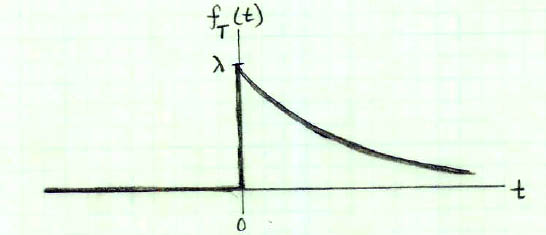
\includegraphics[scale=0.5]{Figure1.jpg}
\end{center}

So, while $\pi_k$ is the \underline{prior} probability that $z_n = k$,
$\gamma_{nk}$ is the \underline{posterior} probability that $z_n = k$
after we have observed $\xb_n$.

Unlike in the case of K-means, where training data points are assigned to a
particular cluster and $N_k$ is the number of points in that cluster, for the
mixture model, we can think of $N_k$ as the ``effective number'' of points in
cluster $k$.

Thus, in equation \eqref{eqn:mu}, $\ub_k$ is a weighted mean of the training
data, where the weights are given by the responsibilities, $\gamma_{nk}$. A
small value of $\gamma_{nk}$ means that cluster $k$ bears little responsiblity
for data point $\xb_n$ and a large value means that it is very repsonsible for
$\xb_n$. \eqref{eqn:mu} is very similar to the cluster update in K-means,
exect that rather than hard assignments to each cluster -- $r_{nk} = 0 \;
\text{or} \; 1$ -- each data point has a soft assignment based on $\gamma_{nk}$.

\subsubsection{Find $\Sb_k$:}
Looking at our handy table of matrix derivatives, we find that for a symmetric
$\frac{\partial}{\partial \mathbf{X}} \Tr\left(\mathbf{X}^{-1} \mathbf{A} \right)
= -\mathbf{X}^{-1} \mathbf{A} \mathbf{X}^{-1}$. Then, applying product and
chain rules, we have
\begin{align*}
  \frac{\partial}{\partial \Sb} \mathcal{N}(\xb \mid \ub, \Sb) &=
    \frac{\partial}{\partial \Sb}
    \left( \frac{1}{(2 \pi)^\frac{D}{2}\left|\Sb\right|^\frac{1}{2}}
              e^{-\frac{1}{2} (\xb - \ub)\tran \Sb^{-1} (\xb-\ub)}\right) \\
  &= \frac{1}{(2 \pi)^\frac{D}{2}} \left (
      e^{-\frac{1}{2} (\xb - \ub)\tran \Sb^{-1} (\xb-\ub)}
      \frac{\partial}{\partial \Sb} \frac{1}{\left|\Sb\right|^\frac{1}{2}} +
      \frac{1}{\left|\Sb\right|^\frac{1}{2}} \frac{\partial}{\partial \Sb}
    e^{-\frac{1}{2} (\xb - \ub)\tran \Sb^{-1} (\xb-\ub)}
    \right) \\
  &= \frac{1}{(2 \pi)^\frac{D}{2}}
    e^{-\frac{1}{2} (\xb - \ub)\tran \Sb^{-1} (\xb-\ub)}
    \Bigg[
      \left(-\frac{1}{2}\frac{\left|\Sb\right|\Sb^{-1}}
                             {\left|\Sb\right|^\frac{3}{2}}
      \right) \\
      &\qquad\qquad\qquad+ \frac{1}{\left|\Sb\right|^\frac{1}{2}}
        \left(-\frac{1}{2} \frac{\partial}{\partial\Sb}
        \Tr\left(\Sb^{-1}(\xb-\ub)(\xb-\ub)\tran\right)\right)
    \Bigg] \\
    &= -\frac{1}{2} \mathcal{N}(\xb \mid \ub, \Sb) \left(
      \Sb^{-1} - \Sb^{-1} (\xb-\ub) (\xb-\ub) \tran \Sb^{-1} \right)
\end{align*}

Thus, we have
\begin{align*}
  \frac{\partial\mathcal{L}}{\partial\Sb_k} &= \sum_{n=1}^N
    \frac{1}{\sum_{j=1}^K \mathcal{N}(\xb_n \mid \ub_j, \Sb_j) \cdot \pi_j}
    \cdot \pi_k \cdot \left(\frac{\partial}{\partial \Sb_k}
                            \mathcal{N}(\xb_n \mid \ub_k, \Sb_k)\right) \\
  &= -\frac{1}{2} \sum_{n=1}^N \gamma_{nk} \left(
    \Sb^{-1} - \Sb^{-1} (\xb-\ub) (\xb-\ub) \tran \Sb^{-1}
  \right) \\
  &=0
\end{align*}
Rearranging,
\begin{align*}
  \Sb^{-1} \sum_{n=1}^N \gamma_{nk}  &=
   \sum_{n=1}^N \gamma_{nk} (\xb-\ub) (\xb-\ub) \tran \Sb^{-1} \\
  \Sb^{-1} N_k &= \Sb^{-1}
    \left(\sum_{n=1}^N\gamma_{nk} (\xb-\ub)(\xb-\ub)\tran\right) \Sb^{-1}
\end{align*}
Front and back multiplying by the covariance matrix, $\Sb$, we have our result
\begin{equation}
  \tcboxmath{\Sb_k = \frac{1}{N_k} \sum_{n=1}^N \gamma_{nk}
  (\xb_n - \ub) (\xb_n - \ub)\tran}.
  \label{eqn:sigma}
\end{equation}
As with the means, this is simply a weighted sample covariance of the training
data.

\subsubsection{Find $\pi_k$:}
Finding a solution for $\pi_k$, the prior probilities of mixture component $k$
is slightly more complicated, because of the constraint that the prior
probabilities must sum to 1. Rather than a set-the-derivative-equal-to-zero
maximization, this is a \textit{constrained} maximization. This can be done
with the Lagrange multiplier technique. Instead of maxizing $\mathcal{L}$, we
maximize

\begin{equation*}
  \mathcal{L}'  = \mathcal{L} + \lambda
    \left( \sum_{k=1}^K \pi_k\right),
\end{equation*}
where $\lambda$ is the Lagrange multiplier who's value we'll discover by
enforcing the constraint on the solution.
\begin{align*}
  \frac{\partial \mathcal{L}'}{\partial \pi_k}
      &= \frac{\partial \mathcal{L}}{\partial \pi_k} + \lambda \\
  &= \sum_{n=1}^N
    \frac{1}{\sum_{j=1}^K \mathcal{N}(\xb_n \mid \ub_j, \Sb_j) \cdot \pi_j}
    \cdot \mathcal{N}(\xb_n \mid \ub_k, \Sb_k) + \lambda \\
    &= \sum_{n=1}^N \frac{\gamma_{nk}}{\pi_k} + \lambda = 0
\end{align*}
Rearranging and multiplying both sides by $\pi_k$,
\begin{gather*}
    \sum_{n=1}^N \gamma_{nk} = - \lambda \cdot \pi_k \\
    \implies \pi_k = \frac{-N_k}{\lambda}
\end{gather*}
Now, we can enforce the constraint that $\sum_{k=1}^K \pi_k = 1$.
\begin{gather*}
    -\frac{\sum_{k=1}^K N_k}{\lambda} = 1 \\
    \implies \lambda = -N
\end{gather*}
Thus,
\begin{equation}
  \tcboxmath{\pi_k = \frac{N_k}{N}}.
  \label{eqn:pi}
\end{equation}
In other words, the prior probability of each mixture component is the effective
fraction of training data for which the component is given responsibility. If
we were doing hard assignment, this would just be the number of points assigned
to the component.

\textbf{Wait a second!} The maximum likelihood parameters given by
\eqref{eqn:mu}, \eqref{eqn:sigma}, and \eqref{eqn:pi} are not actually in
closed form! The resposibilities, $\gamma{nk}$, appear in the right hand sides
of the equations, but depend on the values of the parameters. This suggests an
iterative solution -- using initial guesses of the parameters to estimate the
responsibilities, then recalculating the parameters. This turns out to be an
instance of the \textbf{Expectation Maximization (EM) Algorithm}.

The EM algorithm is a powerful and general method for optimizing the parameters
for models with \textbf{latent variables}. A latent variable is a random
variable defined as part of generative model that represents something that is
\text{not actually observed}. In the clustering mixture model, the $\{z_n\}$ are
latent variables -- unlike the $\{\xb_n\}$, they are never directly observed.

\subsection{EM Algorithm for Gaussian Mixture Model}
\begin{framed}
\begin{description}[%
  before={\setcounter{descriptcount}{0}},%
  ,font=\bfseries\stepcounter{descriptcount}\thedescriptcount.~]
  \item[Initialize] parameters $\ub_k, \Sb_k, \pi_k \forall k \in 1,\ldots,K$.
              (Also need to decide on $K$!)
  \item[E-step:] Evaluate responsibilities given current parameter values
      \begin{equation*}
        \gamma_{nk} = \frac{\mathcal{N}(\xb_n \mid \ub_k, \Sb_k)}
                        {\sum_{j=1}^K \mathcal{N}(\xb_n \mid \ub_j, \Sb_j)}
      \end{equation*}
  \item[M-step:] Re-estimate parameters using the current values of the
    responsibilities
    \begin{align*}
      \ub_k^{\text{new}} &= \frac{1}{N_k} \sum_{n=1}^N \gamma_{nk} \xb_n \\
      \Sb_k^{\text{new}} &= \frac{1}{N_k} \sum_{n=1}^N \gamma_{nk}
            (\xb_n - \ub^{\text{new}}) (\xb_n - \ub^{\text{new}})\tran \\
      \pi_k^{\text{new}} &= \frac{N_k}{N}
    \end{align*}
    where $N_k = \sum_{n=1}^N \gamma_{nk}$.
  \item[Evaluate the log likelihood of training data:]
    \begin{equation*}
      \log \Pr(\{\xb_n\} \mid \theta) =
        \sum_{n=1}^N \log \left[ \sum_{k=1}^K
              \mathcal{N}(\xb_n \mid \ub_k, \Sb_k) \cdot \pi_k \right]
    \end{equation*}
    in order to see whether it has converged. (Alternatively, one can track the
    convergence of the parameters after step \textbf{3}.) If the convergence
    criteria are not satisfied go to step \textbf{2}.
\end{description}
\end{framed}

After each iteration of the EM algorithm the log likelihood of the training
data, $\log \Pr(\{\xb_n\} \mid \theta)$, increases (meaning that the parameter
estimates are improving).

\textbf{Mixtures of Exponential Family Distributions:} We have calculated the
M-step parameter updates for clustering using a mixture of Gaussians model. The
solution ends up being weighted versions of the typical maximum-likelihood
parameter estimates for $\ub_k$ and $\Sb_k$. Here's a conjecture
\begin{conjecture}
  For a mixture model defined using an distribution from the exponential family,
  the parameter updates in the M-step of the EM algorithm will take the form
  of weighted averages of the sample estimates of these parameters.
\end{conjecture}
Here's the outline of a proof.
\begin{proof}
If we consider a distribution in the very general exponential family, we can
define
\begin{equation}
  \Pr(\xb \mid z = k) = f(\xb \mid \symbf{\eta}_k) = h(\xb)
      \exp \left(\symbf{\eta}_k\tran T(\xb) - A(\symbf{\eta}_k)\right)
  \label{eqn:expfamily}
\end{equation}
where $\symbf{\eta}_k$ are the so-called ``natural parameters'' of the
distribution $f(\xb)$ for component $k$. The typical parameters that we think of
may not be the natural ones, but can be simply derived from them. The functions
$h()$, $T()$, and $A()$ are determined by the type of distribution. If we have
some data $\{\xb_n\}$, for a general exponential family distribution, the
maximum likelihood estimates for the natural parameters are the solution to the
equation
\begin{equation*}
  \frac{\partial}{\partial \symbf{\eta}} A(\symbf{\eta}) = \frac{\sum_{n=1}^N T(\xb_n)}{N}.
\end{equation*}
So now let's consider our mixture model.
\begin{equation}
  \frac{\partial\mathcal{L}}{\partial\symbf{\eta}_k} = \sum_{n=1}^N
    \frac{1}{\sum_{j=1}^K f(\xb \mid \symbf{\eta}_j)}
    \cdot \pi_k \cdot \left(\frac{\partial}{\partial\symbf{\eta}_k}
                            f(\xb \mid \symbf{\eta}_k)\right)
\end{equation}
From \eqref{eqn:expfamily}, we can see that
\begin{equation*}
  \frac{\partial}{\partial\symbf{\eta}} f(\xb \mid \symbf{\eta}) =
  f(\xb) \left(T(\xb) - \frac{\partial}{\partial \symbf{\eta}}
    A(\symbf{\eta}) \right)
\end{equation*}
Plugging this in, we have
\begin{gather}
  \frac{\partial\mathcal{L}}{\partial\symbf{\eta}_k} = \sum_{n=1}^N
    \gamma_{nk} \left(T(\xb) - \frac{\partial}{\partial \symbf{\eta}_k}
      A(\symbf{\eta}_k) \right) = 0 \\
  \implies \frac{\partial}{\partial \symbf{\eta}_k} A(\symbf{\eta}_k) =
    \frac{1}{N_k} \sum_{n=1}^N \gamma_{nk} T(\xb).
\end{gather}
Notice that this has the same form as the general maximum likelihood parameter
estimate, but weighted by the responsibilities $\gamma_{nk}$.
\end{proof}

\end{document}
